\section{Red laboratorio}

Para este experimento se tomo una captura de 30 minutos de la red Wi-Fi de los labos de la facultad.

\begin{figure}[h]
  \centering
    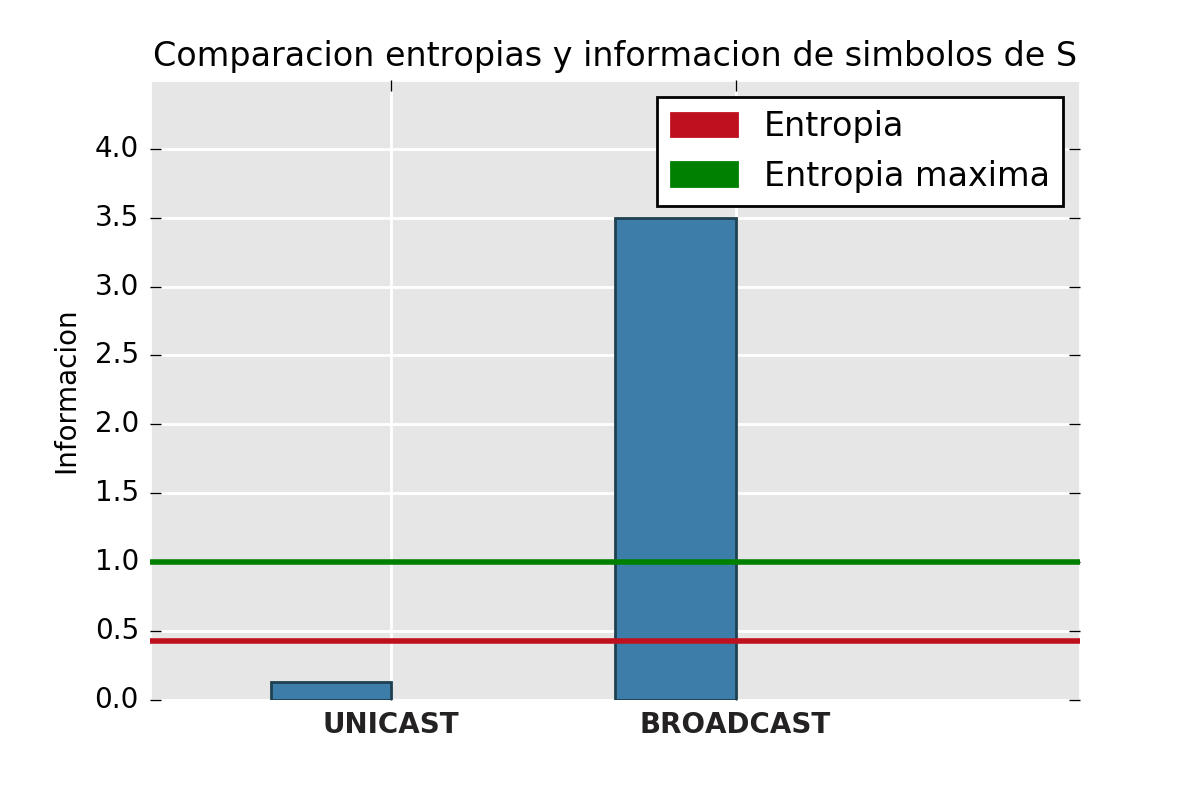
\includegraphics[width=0.45\textwidth]{grafico1-red-labos.png}
  \caption{Entropia de la fuente}
  \label{entropia-s}
\end{figure}

Como podemos ver en el gráfico comparativo la entropía no llega a ser máxima. De hecho puede verse en el símbolo $BROADCAST$ proporciona mucha mas información que el símbolo $UNICAST$. 

Por lo que hay un mayor flujo de paquetes Ethernet $UNICAST$ que $BROADCAST$, esto podría deberse a cambios en la topología de la red.

Dado que esta es una red Wi-fi, se esperaría que haya muchos dispositivos conectandose y desconectandose, con lo cual es muy factible que la topología de la red vaya variando a lo largo del tiempo.

Los cambios de topología redicen el tiempo de las entradas en la tabla CAM en el caso de Spanning Tree Protocol. En redes que hacen uso de Rapid Spanning Tree Protocol, las direcciones MAC se liberan de la tabla CAM de forma inmediata.


    \begin{table}[ht]\begin{center}
      \begin{tabular}{|c|c|}
      \hline
      \textbf{Nodo} & \textbf{Información} \\ \hline
      \texttt{UNICAST}& 0.133654 \\ \hline
      \texttt{BROADCAST}& 3.498507 \\ \hline
      \end{tabular}
      \caption{Información de los símbolos de S}
      \label{info-simbolos}
    \end{center}\end{table}


El overhead impuesto por la red influencia la entropía de esta fuente.
Por ejemplo, si hubiese mas mensajes $ARP$ $BROADCAST$ la información del símbolo $S_{BROADCAST}$ bajaría haciendo consecuentemente que la entropía de la fuente $S$ se vea modificada.

\begin{figure}[h]
  \centering
    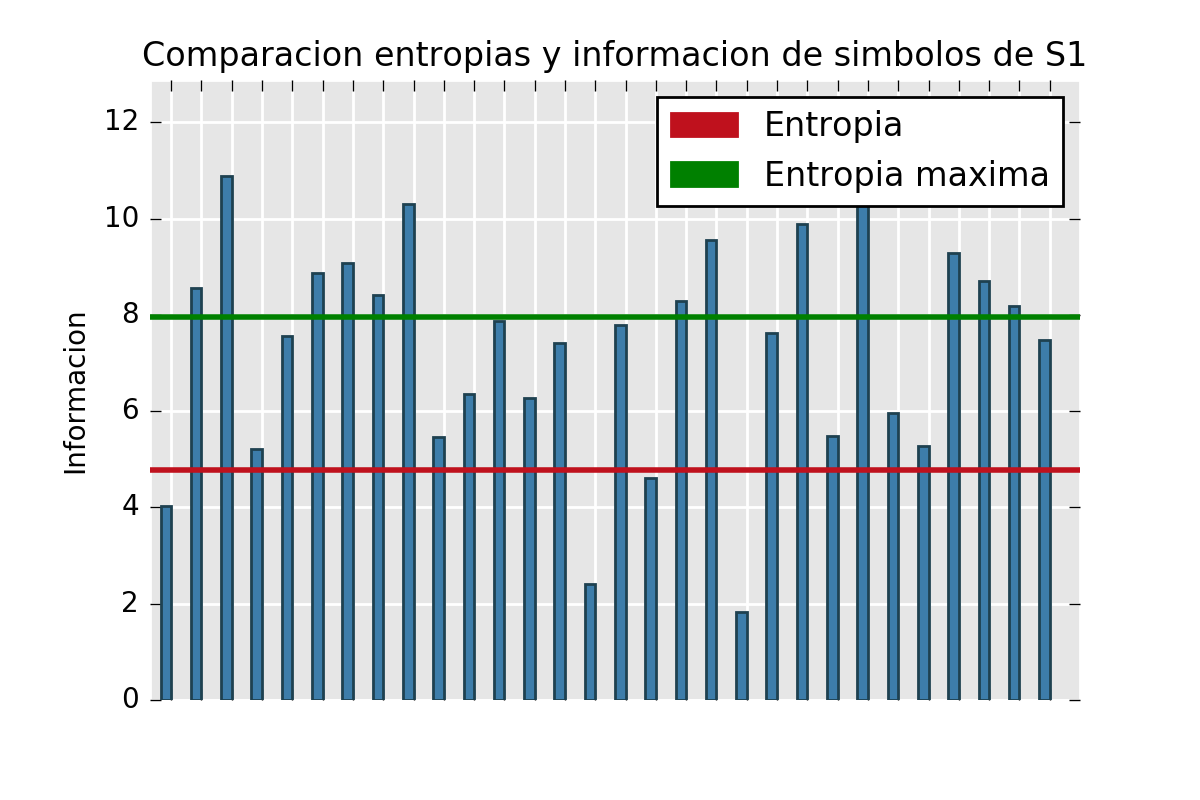
\includegraphics[width=0.45\textwidth]{grafico2-red-labos.png}
  \caption{Entropia de la fuente S1}
  \label{entropia-s1}
\end{figure}
En este gráfico agrupamos la información puesto que había demasiados símbolos.

En comparación con el resto de los mensajes el tráfico $ARP$ es bajo, sólo el 4\% de los mensajes son $ARP$. En base al criterio propuesto, se pueden distinguir 4 nodos, que en el grafico se corresponden con las cuatro barras que están por debajo de la entroppía de la fuente:   

    \begin{table}[ht]\begin{center}
      \begin{tabular}{|c|c|}
      \hline
      \textbf{Nodo} & \textbf{Informacion} \\ \hline
      \texttt{10.2.7.254}& 1.829564 \\ \hline
      \texttt{10.2.203.254}& 2.414527 \\ \hline
      \texttt{10.2.1.250}& 4.026302 \\ \hline
      \texttt{10.2.3.254}& 4.601927 \\ \hline
      \end{tabular}
      \caption{Nodos destacados}
      \label{Nodos-destacados}
    \end{center}\end{table}

Como en nuestra fuente estamos tomando las IPs destino de los paquetes $ARP$ $Who-has$. Esto indíca que estas IPs son muy frecuentes con lo cual se podría pensar en el escenario en que la mayoría de los nodos quiere conocer la MAC del Default Gateway por lo tanto envían tramas $Who-has$ con la dirección destino del mismo.

Por lo tanto bajo ese escenario estos cuatro nodos distinguidos podrían ser Default Gateway/s. 


\begin{figure}[h]
  \centering
    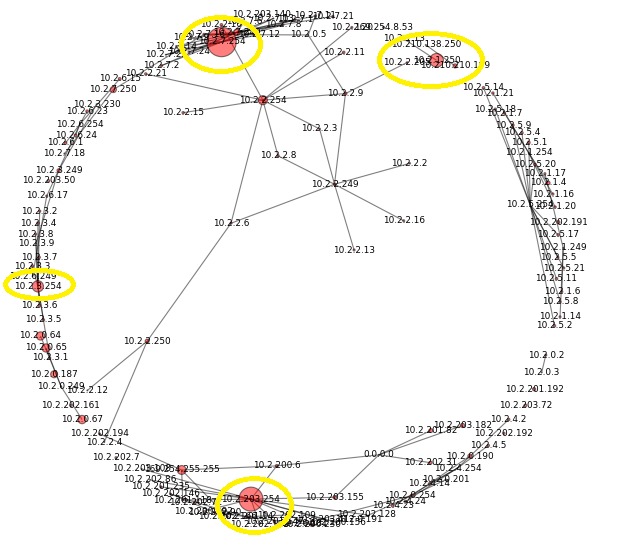
\includegraphics[width=0.45\textwidth]{grafo-red-labos-destacados.png}
  \caption{Grafo de la fuente S1}
  \label{grafo-s1}
\end{figure}
